\chapter{Computing Rectification function}
\label{ch:rectfunc}
Lorem ipsum dolor sit amet, consectetur adipiscing elit. Duis tincidunt eros ut dictum tempor. Proin rhoncus elementum mauris, ac bibendum quam. Sed eget nisi non arcu malesuada pulvinar a at ipsum. Curabitur ante quam, aliquet id purus ac, interdum semper odio. Suspendisse potenti. Aliquam rhoncus massa consectetur faucibus condimentum. Sed euismod tellus eu mattis elementum. In nec laoreet ligula. Donec vel blandit ante. Mauris non ligula non justo venenatis rhoncus. In quis auctor ipsum, in mattis lacus. In vitae lectus sodales arcu iaculis bibendum. Fusce ornare at ex vitae ultricies.

Nullam sagittis maximus leo, sit amet dictum neque suscipit at. Proin sagittis mollis mi, at ornare ligula ornare nec. Donec et pulvinar mi. Nulla ac semper dui, id mollis ante. Nam cursus vel tellus quis maximus. Vestibulum quis nunc sit amet felis mollis facilisis sed a sapien. Sed sit amet nisi velit. Mauris tellus arcu, commodo in feugiat in, porttitor vitae urna. Vivamus in aliquet elit. Nunc quis dui massa. Morbi blandit fringilla dui et fermentum. Nulla facilisi. Aenean et dui turpis. Mauris tempor diam ac mi scelerisque lacinia.

\section{Problem Statement}

\begin{Example}
Consider a buggy 2-bit multiplier in Fig. \ref{fig:mult2_b2}. 

\begin{figure}[H]
    \centering
    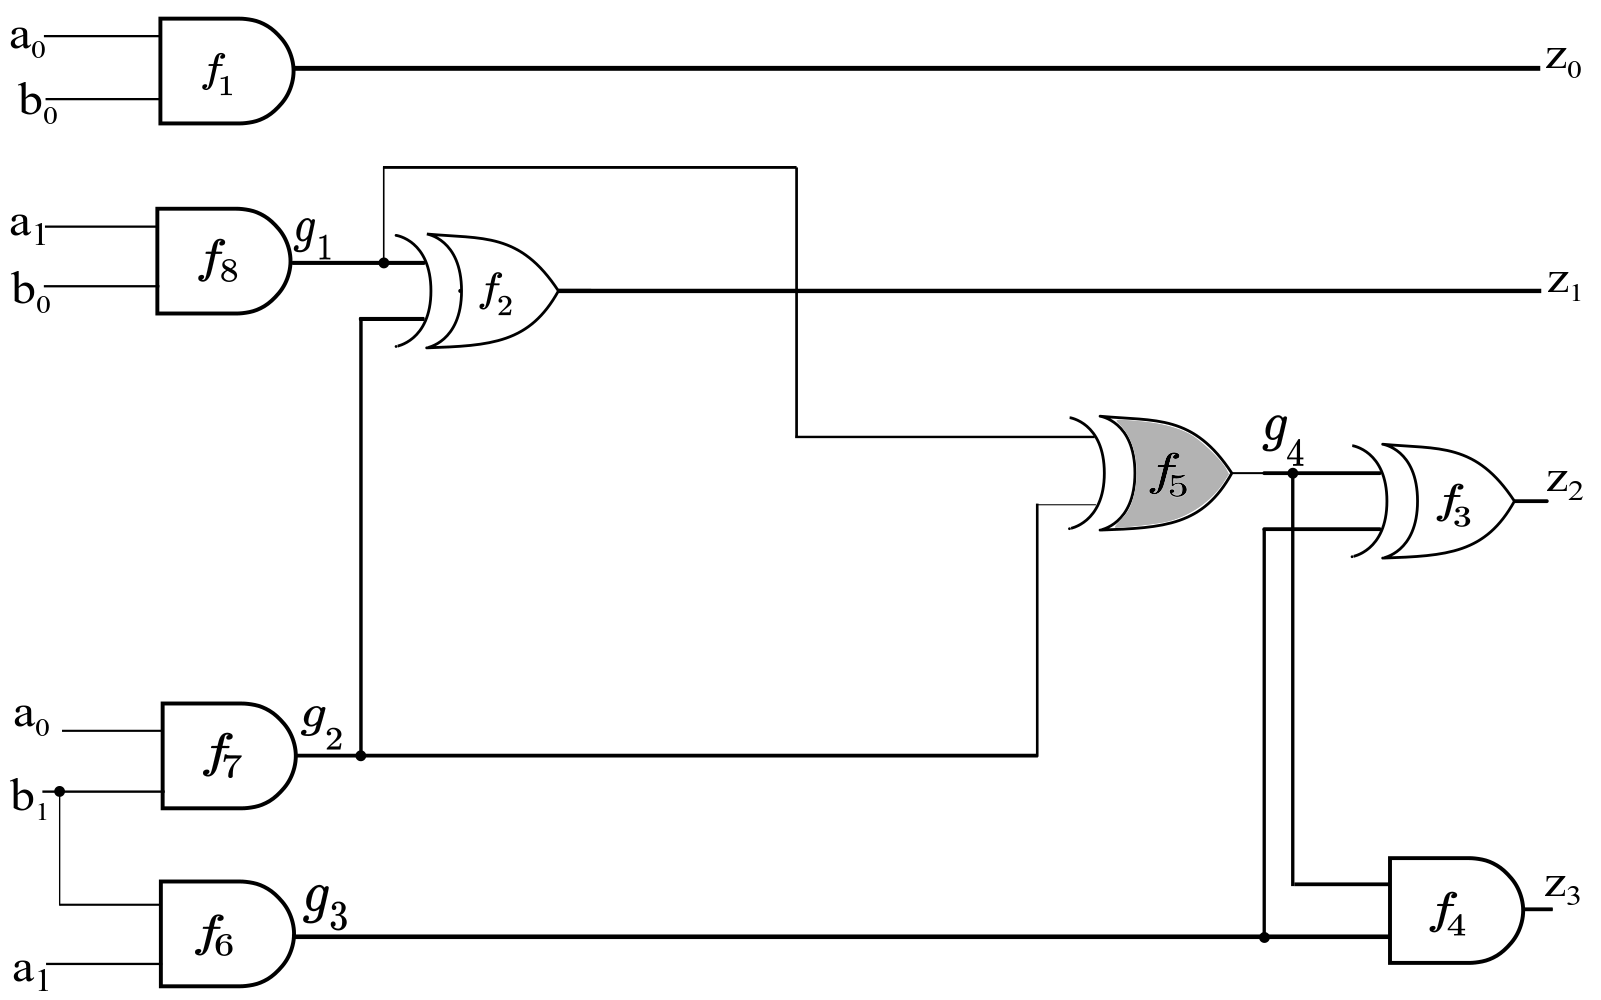
\includegraphics[scale = 0.2]{mult2_b.png}
    \caption{2-bit Integer multiplier with a bug. The AND gate at $g_4$ replaced by an XOR gate.}
    \label{fig:mult2_b2}
\end{figure}

\end{Example}

\section{Computing rectification function}

LLorem ipsum dolor sit amet, consectetur adipiscing elit. Duis tincidunt eros ut dictum tempor. Proin rhoncus elementum mauris, ac bibendum quam. Sed eget nisi non arcu malesuada pulvinar a at ipsum. Curabitur ante quam, aliquet id purus ac, interdum semper odio. Suspendisse potenti. Aliquam rhoncus massa consectetur faucibus condimentum. Sed euismod tellus eu mattis elementum. In nec laoreet ligula. Donec vel blandit ante. Mauris non ligula non justo venenatis rhoncus. In quis auctor ipsum, in mattis lacus. In vitae lectus sodales arcu iaculis bibendum. Fusce ornare at ex vitae ultricies.

Nullam sagittis maximus leo, sit amet dictum neque suscipit at. Proin sagittis mollis mi, at ornare ligula ornare nec. Donec et pulvinar mi. Nulla ac semper dui, id mollis ante. Nam cursus vel tellus quis maximus. Vestibulum quis nunc sit amet felis mollis facilisis sed a sapien. Sed sit amet nisi velit. Mauris tellus arcu, commodo in feugiat in, porttitor vitae urna. Vivamus in aliquet elit. Nunc quis dui massa. Morbi blandit fringilla dui et fermentum. Nulla facilisi. Aenean et dui turpis. Mauris tempor diam ac mi scelerisque lacinia.

\begin{equation}
\label{eq:eqn1}
    f \in \langle f_1,\dots,f_{i-1},\boldsymbol{f_i: x_i - U},f_{i+1},\dots,f_s,x_1^2-x_1,\dots,x_n^2-x_n \rangle
\end{equation}

Lorem ipsum dolor sit amet, consectetur adipiscing elit. Duis tincidunt eros ut dictum tempor. Proin rhoncus elementum mauris, ac bibendum quam. Sed eget nisi non arcu malesuada pulvinar a at ipsum. Curabitur ante quam, aliquet id purus ac, interdum semper odio. Suspendisse potenti. Aliquam rhoncus massa consectetur faucibus condimentum. Sed euismod tellus eu mattis elementum. In nec laoreet ligula. Donec vel blandit ante. Mauris non ligula non justo venenatis rhoncus. In quis auctor ipsum, in mattis lacus. In vitae lectus sodales arcu iaculis bibendum. Fusce ornare at ex vitae ultricies.

Nullam sagittis maximus leo, sit amet dictum neque suscipit at. Proin sagittis mollis mi, at ornare ligula ornare nec. Donec et pulvinar mi. Nulla ac semper dui, id mollis ante. Nam cursus vel tellus quis maximus. Vestibulum quis nunc sit amet felis mollis facilisis sed a sapien. Sed sit amet nisi velit. Mauris tellus arcu, commodo in feugiat in, porttitor vitae urna. Vivamus in aliquet elit. Nunc quis dui massa. Morbi blandit fringilla dui et fermentum. Nulla facilisi. Aenean et dui turpis. Mauris tempor diam ac mi scelerisque lacinia.

\subsection{Procedure to compute rectification function}
\vspace{2mm}
\begin{table}[ht]
    \centering
    \begin{tabular}{|c|c|c|} \hline
      $a_0,a_1,a_2,b_0,b_1,b_2$ & $h_i$ & $h_i'$ \\ \hline
       0,0,0,0,0,0 & -12 & 1\\ \hline
       0,0,0,0,0,1 & -12 & 1\\ \hline
       0,0,0,0,1,0 & -12 & 1\\ \hline
       0,1,0,0,0,1 & 0 & $-\frac{1}{3}$\\ \hline
       0,1,0,0,1,0 & 0 & $\frac{1}{3}$\\ \hline
       0,1,0,0,1,1 & 0 & -1 \\ \hline
    \end{tabular}
    \caption{Evaluating $h_i$ and $h_i'$}
    \label{tab:quosol}
\end{table}

In order to conserve space, Table \ref{tab:quosol} shows the data for only some input patterns. We make some observations based on the contents of this table. 

\section{Conclusion}
Lorem ipsum dolor sit amet, consectetur adipiscing elit. Duis tincidunt eros ut dictum tempor. Proin rhoncus elementum mauris, ac bibendum quam. Sed eget nisi non arcu malesuada pulvinar a at ipsum. Curabitur ante quam, aliquet id purus ac, interdum semper odio. Suspendisse potenti. Aliquam rhoncus massa consectetur faucibus condimentum. Sed euismod tellus eu mattis elementum. In nec laoreet ligula. Donec vel blandit ante. Mauris non ligula non justo venenatis rhoncus. In quis auctor ipsum, in mattis lacus. In vitae lectus sodales arcu iaculis bibendum. Fusce ornare at ex vitae ultricies.

Nullam sagittis maximus leo, sit amet dictum neque suscipit at. Proin sagittis mollis mi, at ornare ligula ornare nec. Donec et pulvinar mi. Nulla ac semper dui, id mollis ante. Nam cursus vel tellus quis maximus. Vestibulum quis nunc sit amet felis mollis facilisis sed a sapien. Sed sit amet nisi velit. Mauris tellus arcu, commodo in feugiat in, porttitor vitae urna. Vivamus in aliquet elit. Nunc quis dui massa. Morbi blandit fringilla dui et fermentum. Nulla facilisi. Aenean et dui turpis. Mauris tempor diam ac mi scelerisque lacinia. 
